\section{PAGRINDINIAI MATŲ ATRINKIMO METODAI}
\label{pagrindiniai_matu_atrinkimo_motodai}

Dėl ,,daugiamatiškumo prakeiksmo`` (angl. \textit{the curse of dimentionality}) didėjant matų kiekiui mėginiai pasidaro panašūs, todėl bandymas juos klasifikuoti tolygus spėliojimui \cite{bellman1966adaptive}. Biomedicininių duomenų kontekste galima daryti prielaidą, kad ne visi matai yra susiję su tiriama problema dėl to, kad duomenys yra daugiamačiai.
%% DJ: Paprastai nagrinėjamai problemai svarbus yra mažas, palyginus su visu, matų kiekis. 
Todėl biomedicininių duomenų daugiamatiškumui sumažinti yra naudojami informatyviausių matų atrinkimo metodai \cite{guyon2003introduction} (angl. \textit{feature selection}). Matų atrinkimas yra svarbi biomedicininių duomenų apdorojimo (angl. \textit{preprocessing}) etapo dalis. Naudojant matų atrinkimo metodus, galima kovoti su daugiamatiškumo prakeiksmu matų skaičių priartinant prie mėginių skaičiaus. Kadangi matų atrinkimo rezultatai priklauso nuo konkrečių duomenų, todėl svarbu yra pasirinkti tinkamiausią matų atrinkimo strategiją

Pagal tai, kaip matų atrinkimo metodai yra susiję su klasifikatoriumi, matų atrinkimo metodus galima skirstyti į tris kategorijas \cite{saeys2008robust}:
\begin{itemize}
 \item Filtruojantys metodai (angl. \textit{filter methods}), pvz. \textit{Fisher} įvertis. Jie dirba tiesiogiai su duomenimis, o jų darbo rezultatas gali būti matų įvertinimas svoriais, matų reitingavimas ar tiesiog geriausių matų poaibis, kuriuo remiantis vėliau apmokomas klasifikatorius. Tokių metodų pagrindinis privalumas yra tai, kad jie yra greiti, tinka paskirstytų skaičiavimų aplinkoms ir nepriklausomi nuo klasifikavimo  metodo, tačiau remiantis atrinktaisiais matais nebūtinai bus sukurtas geriausias klasifikatorius.
 \item Prisitaikantieji metodai (angl. \textit{wrapper methods}). Pirma, apmokomas klasifikatorius su visais matais, antra, parenkamas matų poaibis ir apmokomas klasifikatorius. Po daugkartinio matų poaibių įvertinimo pagal klasifikavimo rezultatus yra nusprendžiama, kuris matų poaibis yra labiausiai tinkamas klasifikavimui. Įterptinių metodų atveju matų atrinkimo procesas yra neatsiejamas nuo klasifikavimo proceso -- matai yra atrenkami pagal klasifikatoriaus darbo rezultatus. Prisitaikantieji metodai dažnai duoda geresnius rezultatus negu filtravimo metodai, bet yra reiklūs resursams.
 \item Įterptiniai metodai (angl. \textit{embedded methods}), pvz. AW-SVM\cite{vapnik2000nature}. Jie matų atrinkimui naudoja vidinius klasifikatoriaus duomenis (pvz. matų svoriai gauti pagal atraminių vektorių klasifikatorius). Šie metodai dažnai siūlo gerą santykį tarp klasifikavimo tikslumo ir skaičiavimų sudėtingumo.
\end{itemize}

Šiame skyriuje yra nagrinėjai pagrindiniai matų atrinkimo metodai: \textit{Fisher} įvertis, \textit{Relief} metodas, asimetrinis priklausomybės koeficientas, absoliučių svorių SVM, rekursyvus matų eliminavimas pagal SVM.

\subsection{\textit{Fisher} įvertis}

\textit{Fisher} įvertis (angl. \textit{Fisher ratio}) vertina individualius matus pagal matų klasių atskiriamąją galią \cite{Pavlidis:2001:GFC:369133.369228}. Mato įvertis yra sudarytas iš atskirų klasių vidurkių skirtumo santykio su klasių standartinių nuokrypių suma:
\begin{equation}
 FR(j) = \frac{(\mu_{j1} - \mu_{j2})^2}{\sigma_{j1}^2 + \sigma_{j2}^2},
\end{equation}
kur, 
$j$ -- mato indeksas, 
$\mu_{jc}$ -- mato $j$ reikšmių vidurkis klasėje $c$, 
$\sigma_{jc}^2$ -- mato $j$ reikšmių standartinis nuokrypis klasėje $c$, kur $c={1,2}$. Kuo didesnis yra \textit{Fisher} įvertis, tuo geriau tas matas atskiria klases. Šis metodas neįvertina matų tarpusavio sąveikų.

\subsection{\textit{Relief} metodas}

\textit{Relief} metodas iteratyviai skaičiuoja matų ,,susietumą``. Pradžioje ,,susietumas`` visiems matams yra lygus nuliui. Kiekvienoje iteracijoje atsitiktinai pasirenkamas mėginys iš mėginių aibės, surandami artimiausi kaimynai iš tos pačios ir kitos klasių, ir atnaujinamos visų matų ,,susietumo`` reikšmės \cite{DBLP:journals/ml/Robnik-SikonjaK03}. Dėl atsitiktinumo faktoriaus klasifikavimo ir  matų atrinkimo stabilumo rezultatai naudojant šį metodą varijuoja. Mato įvertis yra vidurkis visų objektų atstumų skirtumų iki artimiausių kaimynų iš kitos ir tos pačios klasių:
\begin{equation}
 W(j)=W(j) - \frac{diff(j, x, x_H)}{n} + \frac{diff(i, x, x_M)}{n},
\end{equation}
kur 
$W(j)$ -- $j$-ojo mato ,,susietumo`` įvertis, 
$n$ -- mėginių aibės dydis, 
$x$ -- atsitiktinai pasirinktas mėginys, 
$x_H$ - artimiausias $x$ kaimynas iš tos pačios klasės (angl. \textit{nearest-Hit}), 
$x_M$ -- artimiausias $x$ kaimynas iš kitos klasės (angl. \textit{nearest-Miss}),
$diff(j, x, x')$ -- $j$-ojo mato reikšmių skirtumas tarp atsitiktinai pasirinkto mėginio $x$ ir atitinkamo jo kaimyno. Skirtumą į intervalą $[0, 1]$ normalizuojanti funkcija yra:
\begin{equation}
 diff(j, x, x')=\frac{|x_j- x_j'|}{x_{j_{max}} - x_{i_{min}}},
\end{equation}
kur $x_{j_{max}}$ ir $x_{j_{min}}$ yra maksimali ir minimali $j$-ojo mato reikšmės. ,,Susietumo`` reikšmių atnaujinimas yra vykdomas $n$ kartų ir kuo didesnė galutinė reikšmė, tuo svarbesnis matas. Šis algoritmas atsižvelgia į matų tarpusavio priklausomybes, nes mėginio artimiausias kaimynas yra ieškomas pagal visus mėginį apibūdinančius matus. Aprašyta algoritmo versija yra skirta dviejų klasių atvejui, tačiau yra ir multiklasinis algoritmo variantas \cite{DBLP:journals/ml/Robnik-SikonjaK03}.

\subsection{Asimetrinis priklausomybės koeficientas}

Asimetrinis priklausomybės koeficientas (angl. \textit{Asymetric Dependency Coefficient}, ADC) yra matų reitingavimo motodas, kuris matuoja mėginio klasės tikimybinę priklausomybę nuo $j$-ojo mato, naudodamas informacijos prieaugio metriką (angl. \textit{information gain}) \cite{Shannon:2001:MTC:584091.584093}:
\begin{equation}
 ADC(Y, j) = \frac{MI(Y, X_j)}{H(Y)},
\end{equation}
kur $H(Y)$ -- klasės $Y$ entropija (angl. \textit{entropy}), o $MI(Y, X_j)$ -- yra tarpusavio informacija (angl. \textit{mutual information}) tarp mėginio klasės $Y$ ir $j$-ojo mato \cite{kent1983information}.
\begin{equation}
 H(Y)=-\sum_y{p(Y=y)log{p(Y=y)}}, 
\end{equation}
\begin{equation}
 H(X_j)=-\sum_x{p(X_j=x) log{p(X_j=x)}},
\end{equation}
\begin{equation}
 MI(Y, X_j) = H(Y) + H(X_j) - H(Y, X_j),
\end{equation}
\begin{equation}
 H(Y, X_j) = -\sum_{y,x_j}{p(y, x_j)log{p(y, x_j)}},
\end{equation}
Kuo didesni ADC įverčiai, tuo matas yra svarbesnis, nes turi daugiau informacijos apie mėginio priklausomybę klasei.

\subsection{Absoliučių svorių SVM}

Viena priežasčių, kodėl atraminių vektorių klasifikatoriai (SVM) yra vienas populiariausių klasifikavimo algortimų, yra tai, kad jis gerai susidoroja su daugiamačiais duomenimis \cite{guyon2002gene}. Yra keletas bazinių SVM variantų, bet šiame darbe naudojamas tiesinis SVM, nes jis demonstruoja gerus rezultatus analizuojant genų ekspresijos duomenimis \cite{vapnik2000nature}. Tiesinis SVM yra hiperplokštuma apibrėžta kaip:
\begin{equation}
 \sum_{j=1}^{p}{w_jx_j + b_0 = 0},
\end{equation}
kur $p$ -- matų kiekis, $w_j$ -- j-ojo mato svoris, $x_j$ -- j-ojo mato kintamasis, $b_0$ -- sisteminis nuokrypis. Mato absoliutus svoris $w_j$ gali būti panaudotas
matų reitingavimui. Svorį reikia imti absoliutaus dydžio, nes neigiamas svoris implikuoja priklausomybę vienai grupei, o teigiamas kitai grupei. Todėl metodas ir vadinamas absoliučių svorių SVM (angl. \textit{Absolute Weight SVM}, AW-SVM). Pastebėtina, kad svorių nustatymas yra atliekamas tik vieną kartą (SVM-RFE matų atrinkimo metodas svorius matams nustato daug kartų).

\subsection{Rekursyvus matų eliminavimas pagal SVM}

Rekursyvus matų eliminavimas pagal SVM (angl. \textit{Support Vector Machines -- Recursive Feature Elimination}, SVM-RFE) yra vienas populiariausių matų atrinkimo algoritmų \cite{guyon2002gene}. Todėl, jis yra naudojamas kaip atskaitos taškas (angl. \textit{benchmark}) vertinant kitus matų atrankimo metodus. Iš esmės šis metodas yra daugkartinis absoliučių svorių SVM metodo taikymas nuolat išmetinėjant matus su mažiausiais svoriais. Rekursyvus matų eliminavimas mums padeda surasti klasifikavimui tinkamą matų poaibį, kas ne visada pavyksta su matų reitingavimo metodais. Rekursyvus matų eliminavimas yra aprašytas algoritme nr. \ref{RFE}.
\begin{algorithm}
\caption{Rekursyvus matų eliminavimas}
\label{RFE}
 \begin{enumerate}
 \item Turime pilną matų rinkinį $F_0$, nustatome $i=0$;
 \item Įvertiname kiekvieno mato kokybę matų aibėje $F_i$;
 \item Išmetame mažiausiai kokybišką matą iš $F_I$ tam, kad gautume matų rinkinį $F_{i+1}$;
 \item Nustatome $i=i+1$ ir grįžtame į antrąjį žingsnį kol nėra patenkinta algoritmo pabaigos sąlyga.
\end{enumerate}
\end{algorithm}
Jei trečiajame algoritmo žingsnyje iš matų aibės yra pašalinamas tik viena matas, tai gaunamas matų reitingavimą, o jei pašalinamas fiksuotas skaičius ar dalis (pvz. 50\%) matų, tai matų reitingavimas negaunamas. Pastebėtina, kad rekursyvus matų eliminavimas labai padidina algoritmo sudėtingumą. Algoritmo pabaigos sąlyga gali būti koks nors konkretus matų skaičius arba tiesiog matų aibę mažinama tol, kol visi matai yra išmetami.

\newpage
\section{STABILIŲ MATŲ ATRINKIMO METODAI}
\label{stabiliu_matu_atrinkimo_metodai}

Naudodami matų atrinkimo metodus, biomedicininius duomenis tiriantys mokslininkai susiduria su atrinktųjų matų aibės stabilumo problema -- atrenkant matus pagal kitą mėginių poaibį, gaunamas kitas informatyviausių matų poaibis. Matų atrinkimo nestabilumas yra sąlygotas šių veiksnių:
\begin{enumerate}
 \item Duomenys yra triukšmingi ir kai kurie matai gali būti palaikyti informatyviais dėl atsitiktinių priežasčių;
 \item Daugiamačiuose duomenyse dalis matų koreliuoja, todėl, kuris iš koreliuojančių matų bus pasirinktas, priklauso nuo to, kuriuos mėginius pasirinksime klasifikatoriaus apmokymui;
 \item Kiekvienas matų atrinkimo algoritmas daro skirtingas prielaidas apie tai, kurie matai yra informatyvūs.
\end{enumerate}
Skirtingi metodai tiems patiems duomenims gali atrinkti skirtingus matus. Taip pat, suskaidžius turimus duomenis į atskiras persidengiančias aibes ir atrinkus tą patį kiekį matų tuo pačiu metodu, gaunamos skirtingos matų aibės. Kuo triukšmingesni duomenys, kuo mažiau turima mėginių ir kuo daugiau yra matų, tuo ryškesnė yra ši problema \cite{loscalzo2009consensus}. 

Stabilių matų atrinkimo problematika yra populiarėjanti tyrimų kryptis. Stabilumas aktualus, nes biomedicininiuose duomenyse konkrečiai problemai aktualūs yra tik tam tikri matai. Todėl dalykinės srities ekspertams yra svarbu naudoti tuos matų atrinkimo metodus, kurie atrenka stabilius ir susijusius su analizuojama problema matus. 

Vienas iš būdų didinti matų atrinkimo stabilumą galėtų būti multikriterinių matų atrinkimo metodų naudojimas. Multikriterinių matų atrinkimo metodų esmė yra panaudoti kelis matų atrinkimo metodus suliejant jų rezultatus į vieną bendrą rezultatą. Yra skiriamos trys priežastys, kodėl keletas agreguotų silpnų ir nestabilių matų atrinkimo metodų gali duoti stabilesnius matų atrinkimo rezultatus \cite{dietterich2000ensemble}:
\begin{enumerate}
 \item Keletas skirtingų, bet vienodai gerų hipotezių gali būti teisingos, todėl kriterijų kombinavimas sumažiną tikimybę, kad bus pasirinkta neteisinga hipotezė;
 \item Atskiri matų atrinkimo metodai gali dirbti skirtinguose lokaliuose optimumuose, o kombinavimas gali geriau reprezentuoti tikrąją duomenis generuojančią funkciją;
 \item Kombinuojant keletą kriterijų praplečiama galimų hipotezių erdvė. Todėl, jei pavieniai pagal pavienius kriterijus nerandama teisinga hipotezė, tai kombinuojant keletą kriterijų didėja tikimybė pasirinkti teisingą hipotezę.
\end{enumerate}
Suliejant keletą skirtingų matų atrinkimo metodų rezultatų suliejamos gerosios pavienių matų atrinkimo metodų savybės, taip kompensuojant metodų silpnybes.

Šiame skyriuje aptariama stabilumo matavimų problematika bei matų atrinkimo stabilumą didinantys metodai: svoriais grįstas multikriterinis suliejimas, reitingais grįstas multikriterinis suliejimas, svoriais ir reitingais grįstas multikriterinis suliejimas, multikriterinis rekursyvus matų eliminavimas, konsensuso grupėmis grįstas stabilių matų atrinkimo metodas.

\subsection{Matų atrinkimo stabilumas}

Matų atrinkimo metodų stabilumas gali būti apibrėžtas kaip matų atrinkimo rezultatų variacijų lygis dėl mažų pakeitimų duomenų rinkinyje. Pakeitimai duomenų rinkinyje gali būti mėginių lygio (pvz. mėginiai pridedami arba atimami), matų lygio (pvz. pridedant matams triukšmo) ar abiejų lygių kombinacija.

Svarbu tai, kad matų stabilumas nėra matuojamas nepriklausomai -- jis yra matuojamas atsižvelgiant į klasifikavimo rezultatus. Matuoti stabilumą verta tada, kai pagal atrinktus matus sukuriamas tikslus klasifikatorius.

\subsubsection{Stabilumo vertinimas}

Vertinant matų atrinkimo metodų stabilumą yra svarbu kaip panašiai yra atrenkami matai, kai yra atliekamas matų atrinkimas su vis kitu mėginių ar matų poaibiu. Kuo mažiau skiriasi atrinktoji matų aibė darant pakeitimus duomenyse, tuo matų atrinkimo stabilumas yra didesnis. Vidutinis matų atrinkimo stabilumas gali būti apibrėžtas kaip vidurkis visų reitingavimo metu gautų atrinktų matų poaibių porų tarpusavio panašumo įverčių \cite{kalousis2007stability}:
\begin{equation}
 S_{tot}=\frac{2\sum_{i=1}^{k-1}\sum_{j=i+1}^{k} S(f_i, f_j)}{k*(k-1)},
\end{equation} 
kur $k$ žymi kiek kartų buvo imtas skirtingas mėginių poaibis matų atrinkimui,
$f_i$, $f_j$ -- matų atrinkimo rezultatas -- reitingai, 
$S(f_i, f_j)$ -- aibių panašumo įvertinimo funkcija.

Matų atrinkimo stabilumo įvertis priklauso nuo to, kokią aibių panašumo funkciją naudosime. Tradicinės panašumo įvertinimo funkcijos (persidengimo procentas, \textit{Pearson} koreliacija, \textit{Spearman} koreliacija) yra linkusios priskirti didesnes panašumo reikšmes, kai pasirenkamas didesnis matų poaibis, nes imant didesnį matų poaibį padidėja tikimybė tiesiog atsitiktinai pasirinkti matą.

\subsubsection{\textit{Kuncheva} indexas}

\textit{Kuncheva} indexas \cite{DBLP:conf/aia/Kuncheva07} yra funkcija skirta matuoti aibių panašumui. Ši funkcija gerai tinka matuoti matų atrinkimo atabilumą, nes atsižvelgia į paimto matų poaibio dydį. \textit{Kuncheva} indeksas:
\begin{equation}
\label{kuncheva_index}
 KI(f_i, f_j)=\frac{r*N - s^2}{s*(N-s)}=\frac{r - (s^2/N)}{s - (s^2/N)},
\end{equation}		
kur $s=|f_i|=|f_j|$ yra atrinktų matų aibės dydis, $r=|f_i \bigcap f_j|$ - abiems atrinktiems matų poaibiams bendrų matų skaičius, $N$ - bendras  duomenų aibės matų skaičius. Pastebėtina, kad formulėje esantis atėminys $s^2/N$ ištaiso sisteminį nuokrypį atsirandantį dėl galimybės atsitiktinai pasirinkti matus. 

\textit{Kuncheva} indeksas gali įgyti reikšmes iš intervalo $[-1, 1]$, kur didesnė reikšmė reiškia didesnį panašumą, o artimos nuliui reikšmės reiškia, kad matai atrenkami beveik atsitiktinai.

%% DJ: Kunchevos indekso ypatybė yra ta, kad jis atsižvelgia tik į persidengiančius, tačiau visiškai nekreipia dėmesio į koreliuojančius matus.

\subsubsection{\textit{Jaccard} indeksas}

Vienas paprasčiausi aibių panašumo įverčių yra \textit{Jaccard} indeksas \cite{jaccard1901etude}. \textit{Jaccard} indexas yra santykis tarp aibių sankirtos ir aibių sąjungos:
\begin{equation}
\label{jaccard_index}
 JI(f_i, f_j)=\frac{|f_i \bigcap f_j|}{|f_i \cup f_j|}=\frac{\sum_{l}I(f_i^l=f_j^l=1)}{\sum_{l}I{f_i^l+f_j^l > 0)}}, 
\end{equation}
kur $f_i$ ir $f_j$ yra matų reitingai, $I(x)$ - funkcija grąžinanti 1, jei $x=TRUE$, ir 0 kitu atveju.

\subsubsection{\textit{Hamming} atstumas}

Informacijos teorijoje \textit{Hamming} atstumas \cite{hamming1950error} tarp dviejų vienodo ilgio vektorių yra apibrėžtas kaip pozicijų skaičius, kuriose esantys simboliai nesutampa. \textit{Hamming} atstumas yra minimalus skaičius pakeitimų, kad vieną vektorių padarytume lygų kitam. 
\begin{equation}
\label{hamming_distance}
 HD(X, Y)= \sum_{i=1}^{n} (x_i \oplus y_i),
\end{equation}
kur $\oplus$ - sumos moduliu 2 arba XOR operacija.

Šiuo metodu matuojant matų atrinkimo stabilumą, prieš atstumo matavimą reikia atlikti rezultatų pertvarkymą: pirma, iš atrinktų matų vektorių padaryti bendro matų skaičiaus ilgio binarinius vektorius; antra, vektoriaus elementus, kurių indeksai gaunami matų atrinkimo metodu, nustatyti lygius vienetui. Atlikus tokius pertvarkymus galima matuoti atstumą tarp dviejų matų atrinkimo rezultatų.

\subsection{Svoriais grįstas multikriterinis suliejimas}

Svoriais grįsto multikriterinio matų atrinkimo suliejimo pagal svorius algoritmo pirmajame žingsnyje kiekvienas bazinis metodas priskiria duomenų rinkinio matams svorius, tada tie svoriai yra kombinuojami į vieną sutarties (angl. \textit{consensus}) svorių vektorių, kurio pagrindu yra gaunami matų reitingai. Algoritmas yra pavaizduotas ~\ref{fig:figure4} pav.
\begin{figure}
 \centering
 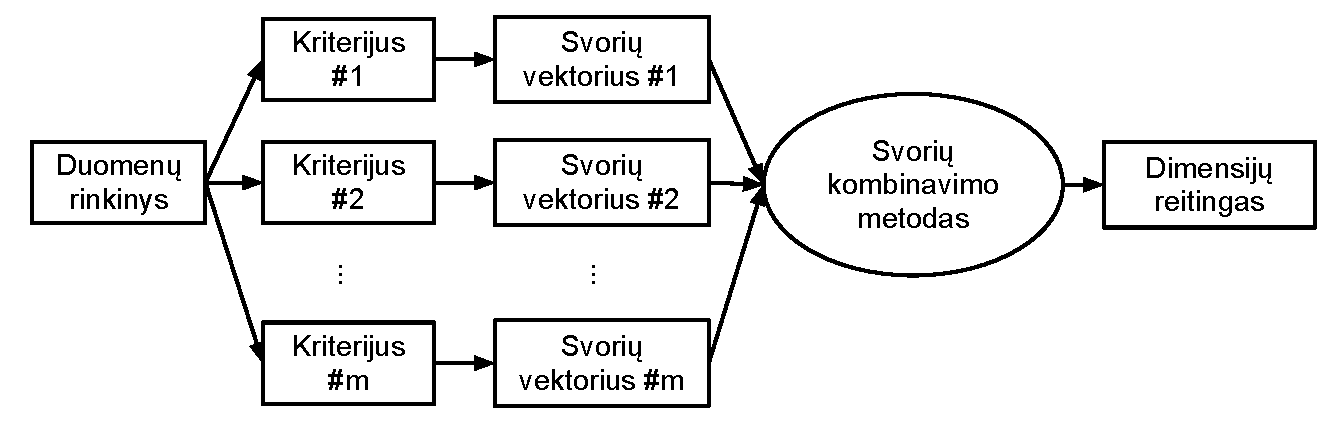
\includegraphics[width=1\textwidth]{images/score_based_fusion.pdf}
 \caption{Svoriais grįstas multikriterinis suliejimas.}
 \label{fig:figure4}
\end{figure}

\begin{figure}[ht]
\begin{minipage}[b]{0.45\linewidth}
\centering
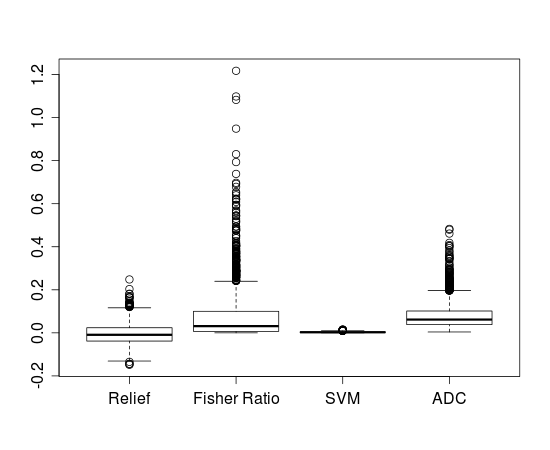
\includegraphics[width=1\textwidth]{images/boxplot_colon_all.png}
\caption{Pavienių matų atrinkimo metodų nenormalizuotas svorių pasiskirstymas.}
\label{fig:figure1}
\end{minipage}
\hspace{0.2cm}
\begin{minipage}[b]{0.45\linewidth}
\centering
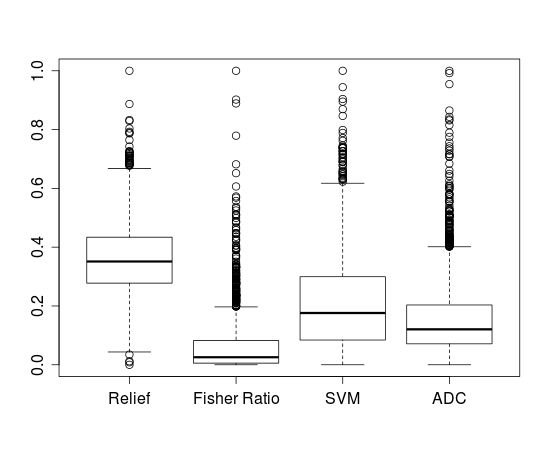
\includegraphics[width=1\textwidth]{images/boxplot_colon_all_normalized.png}
\caption{Pavienių matų atrinkimo metodų normalizuotas svorių pasiskirstymas.}
\label{fig:figure2}
\end{minipage}
\end{figure}

Suliejant svorius svarbu yra užtikrinti, kad svoriai, gauti naudojant skirtingus bazinius kriterijus, būtų palyginami. Todėl svorių normalizavimas turi būti atliekamas prieš svorių kombinavimą. Kitu atveju matų svoriai yra nepalyginami. Paveikslėlyje \ref{fig:figure1} pav. nenormalizuotų pavienių matų vertinimo metodų skiriasi suteiktų svorių intervalai. Paveikslėlyje \ref{fig:figure2} pav. pavaizduota, kad normalizavus matų svorius pastebimai skiriasi svorių kvartiliai -- į tai reikia atkreipti dėmesį interpretuojant galutinius matų vertinimo rezultatus. Svorių normalizavimas į intervalą $[0, 1]$ atliekamas pagal formulę:
\begin{equation}
 u_i'=\frac{u_i - u_{i_{min}}}{u_{i_{max}} - u_{i_{min}}}, 
\end{equation}
kur $u_i$ -- matų svorių vektorius pagal $i$ kriterijų, 
$u_{i_{min}}$ -- minimali $u_i$ svorių vektoriaus reikšmė,
$u_{i_{max}}$ -- maksimali $u_i$ svorių vektoriaus reikšmė,
$u_i'$ -- normalizuotų svorių vektorius.

Sutarties svorių vektorius $u$ yra vidurkis normalizuotų svorių vektorių:
\begin{equation}
 u = \frac{1}{m}\sum_{i=1}^m u_i',
\end{equation}
kur $m$ yra bazinių kriterijų skaičius. Didesnė svorio reikšmė reiškia, kad matas yra reikšmingesnis klasifikavimui.

\subsection{Reitingais grįstas multikriterinis suliejimas}

Reitingais grįsto multikriterinio suliejimo pagal reitingus metodas gauna mėginių aibę aprašančių matų reitingą, pagal keletą bazinių matų reitingavimo kriterijų. Algoritmo pirmajame žingsnyje keletas matų atrinkimo kriterijų grąžina matų reitingus, paskui tie reitingai yra kombinuojami į vieną bendra matų reitingą. Algoritmas yra
pavaizduotas ~\ref{fig:figure5} pav.
\begin{figure}
 \centering
 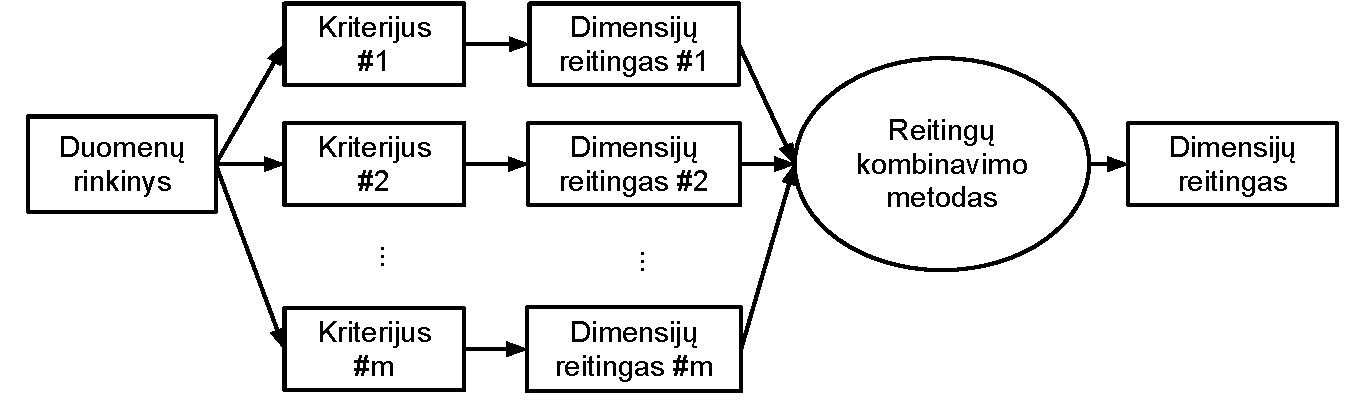
\includegraphics[width=1\textwidth]{images/ranking_based_fusion.pdf}
 \caption{Reitingais grįstas multikriterinis suliejimas.}
 \label{fig:figure5}
\end{figure}
Suliejimo pagal reitingus metodas nereikalauja matų atrinkimo metodų rezultatų normalizavimo, todėl galima matams priskirtus reitingus kombinuoti iškart. Skirtingai nei suliejimo pagal svorius algoritme, baziniai matų atrinkimo kriterijai turi gražinti matų reitingus, o ne svorius.

Matų reitingų kombinavimui yra keletas metodų\cite{dwork2001rank}, tačiau dėl paprastumo naudojamas \textit{Borda} balsavimas\footnote{Dar žinomas kaip ,,Pažymių metodas``. Jis buvo pasiūlytas prancūzų matematiko ir fiziko \textit{Jean-Charles de Borda} 1770 metais.} (angl.\textit{ Borda count}). Tarkime, kad turime $m$ basuotojų ir $p$ kandidatų aibę. Tada Borda balsavimo metodas kiekvienam $i$-ajam balsuotojui sukuria balsų vektorių $v_i$ tokiu būdu: geriausiai įvertintam kandidatui suteikiama $p$ taškų, antrajam kandidatui $p-1$, ir t.t. Galutiniai taškai yra gaunami sudedant visų balsuotojų taškus
\begin{equation}
 v = \sum_{i=1}^m v_i,
\end{equation}
kur $v$ yra suminių taškų vektorius, o iš jo galime gauti ir galutinius matų reitingus.

\subsection{Svoriais ir reitingais grįstas multikriterinis suliejimas}

Svoriais ir reitingais grįsto multikriterinio suliejimo metodas nuo reitingais grįsto multikriterinio suliejimo metodo skiriasi tuo, kad kaip dar vienas matų reitingas yra panaudojamas svoriais grįsto multikriterinio matų atrinkimo metu gautas reitingas. Algoritmas pavaizduotas ~\ref{fig:figure3} pav. Multikriterinis matų atrinkimas pagal svorius ir pagal reitingus atliekamas trimis etapais:
\begin{enumerate}
  \item Gaunamas matų reitingus pagal $m$ pavienių matų atrinkimo motodų;
  \item Suliejamas matų įverčius pagal svorius, taip gaunamas vieną matų reitingą;
  \item Reitinguojami matai pagal visus turimus $m+1$ pavienius reitingus.
\end{enumerate} 
\begin{figure}
 \centering
 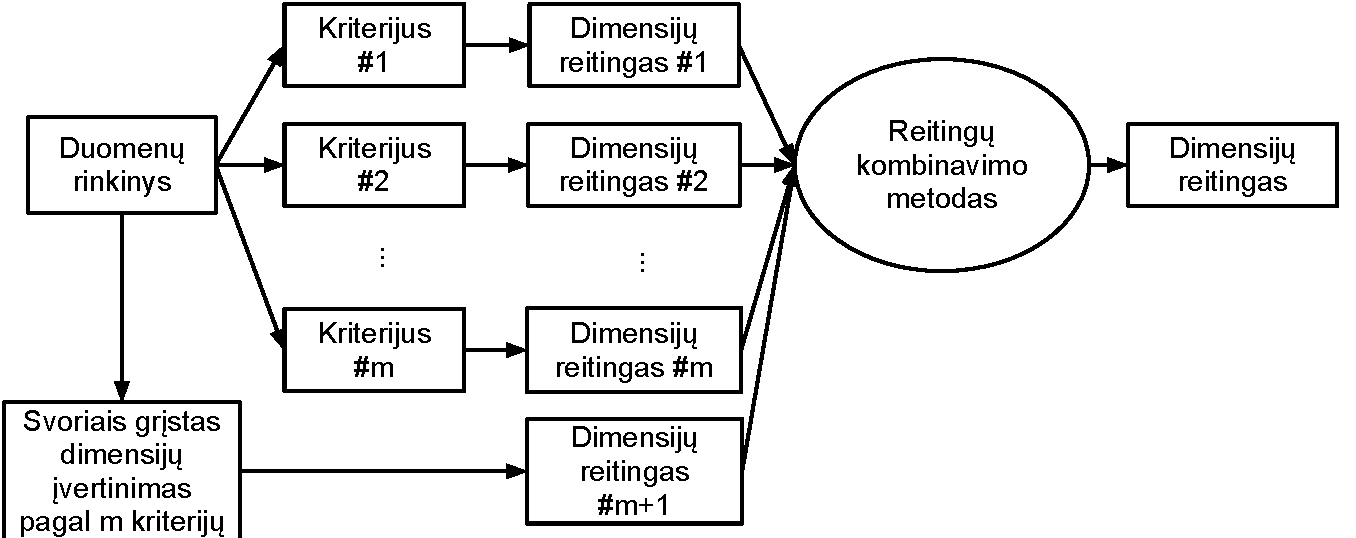
\includegraphics[width=1\textwidth]{images/score_and_ranking_based_fusion.pdf}
 \caption{Svoriais ir reitingais grįstas multikriterinis suliejimas.}
 \label{fig:figure3}
\end{figure}

Suliejant keletą silpnai koreliuojančių matų reitingavimo metodų rezultatų, yra siekiama didesnio matų atrinkimo stabilumo, kai varijuoja treniravimosi duomenų poaibis (angl. \textit{subsampling}) \cite{yang2011robust}.

\subsection{Multikriterinis rekursyvus matų eliminavimas}

Jei matų atrinkimo tikslas yra pagerinti klasifikavimo rezultatus, tai taikant multikriterinius matų atrinkimo metodus nebūtinai surandamas geriausias matų poaibis. Tam, kad būtų surastas geriausias matų poaibis reikia kombinuoti multikriterinį matų reitingavimą su matų paieškos strategija. Rekursyvus matų eliminavimas yra dažnai naudojama paieškos strategija matų atrinkimui. 
%% DJ: Todėl yra kombinuojamas multikriterinis matų reitingavimas ir rekursyvus matų eliminavimas.

Multikriterinis rekursyvus matų eliminavimas (angl. \textit{Multicriterion Fusion Based Recursive Feature Elimination}, MCF-RFE) susideda iš dviejų dalių \cite{yang2011robust}: keleto matų atrinkimo kriterijų suliejimo pagal svorius ir pagal reitingus, ir rekursyvaus matų eliminavimo aprašyto algoritme nr. \ref{RFE}. Algoritmas pavaizduotas ~\ref{fig:figure6} pav.
\begin{figure}
 \centering
 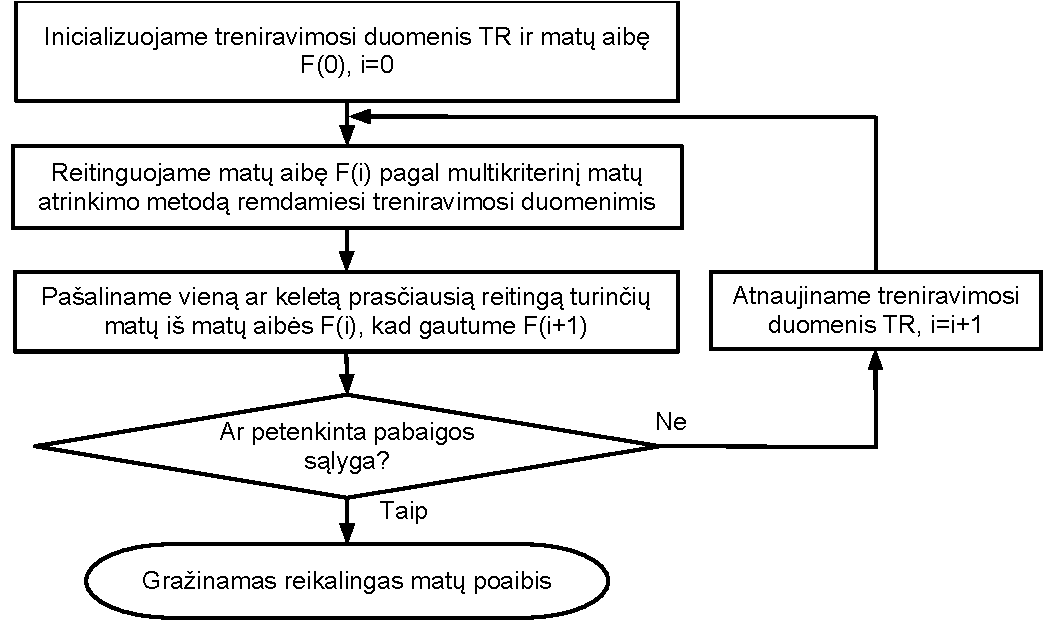
\includegraphics[width=0.7\textwidth]{images/mcf-rfe_procedure.pdf}
 \caption{Multikriterinio rekursyvaus matų eliminavimo algoritmas.}
 \label{fig:figure6}
\end{figure}

Standartinis rekursyvus matų eliminavimas, kai vienos iteracijos metu yra eliminuojamas vienas matas, gali labai padidinti algoritmo sudėtingumą. Todėl genų ekspresijos duomenims prasmingiau yra eliminuoti keletą matų vienu metu.

Nors SVM-RFE matų atrinkimo algoritmas ir yra labai populiarus, tačiau yra žinoma, kad jam trūksta stabilumo \cite{guyon2002gene}. Todėl kombinuodami didesnį stabilumą turintį multikriterinį matų atrinkimą su rekursyvaus matų eliminavimo paieškos strategija, gauname stabilesnį matų atrinkimo algoritmą.

\subsection{Konsensuso grupėmis grįstas stabilių matų atrinkimo metodas}

Konsensuso grupėmis grįstas stabilių matų atrinkimo metodas (angl. \textit{Consensus Group Stable feature selection}, CGS), pirma, identifikuoja tankias matų grupes, antra, pagal surastas grupes transformuoja matų erdvę, trečia, transformuotoje matų erdvėje atlieka matų atrinkimą \cite{loscalzo2009consensus}. Schematiškai šis algoritmas pavaizduotas ~\ref{fig:figure7} pav. 
\begin{figure}
 \centering
 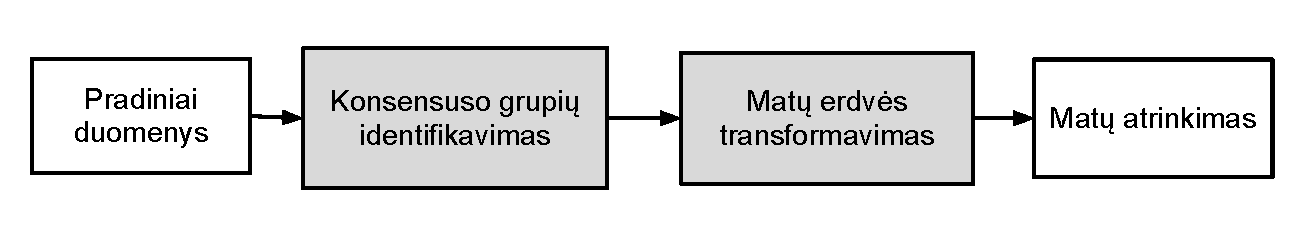
\includegraphics[width=\textwidth]{../bachelor/images/consensus_group_based_feature_selection_framework.pdf}
 \caption{Konsensuso grupėmis grįstas stabilių matų atrinkimas.}
 \label{fig:figure7}
\end{figure}

CGS metodo pagrindinė dalis yra tankių matų identifikavimas. Šio uždavinio sprendimui naudojamas \textit{Dense Group Finder} (DGF) algoritmas. DGF aprašytas algoritme nr. \ref{DGF}. CGS algoritme matai pagal DGF algoritmą yra sugrupuojami keletą kartų. Po pakartotinio grupavimo yra ieškoma stabilių grupių -- jei matas buvo sugrupuotas į konkrečią grupę daugiau nei pusėje grupavimų, tai matas ir priklausys tai konsensuso grupei. Matų aibės transformavimas vyksta iš kiekvienos konsensuso grupės išrenkant reprezentatyviausią matą -- konkretų matą esantį arčiausiai konsensuso grupės vidurkio. Išrinktieji reprezentatyviausieji matai ir sudaro transformuotą matų erdvę. Transformuotoje matų erdvėje vykdomas matų atrinkimas kuriuo nors matų atrinkimo metodu $\Phi$, pvz., \textit{Relief} matų atrinkimo metodu. 
\begin{algorithm}
\caption{DGF -- \textit{Dense Group Finder}}
\label{DGF}
 \begin{algorithmic}
 \item \textbf{Įeitis:} duomenys $D=\{x_i\}_{i=1}^n$, branduolio plotis $h$
 \item \textbf{Išeitis:} tankios matų grupės $G_1, G_1,..., G_L$
 \For{$i = 1$ \textbf{to} $n$ \do} 
  \State Inicializuojame $j=1, y_{i,j}=x_i$
  \Repeat
    \State Suskaičiuoti tankio centrą $y_{i, j+1}$ pagal (\ref{for_dgf})
  \Until{konverguoja}
  \State Nustatyti tankio centrą $y_{i,c} = y_{i,j+1}$ (Nustatyti piką $p_i$ kaip $y_{i,c}$)
  \State Sulieti piką $p_i$ su artimiausiais pikais, jei atstumai tarp jų $ < h$
 \EndFor
 \item Iš kiekvieno unikalaus piko $p_r$, pridėkime $x_i$ į $G_r$, jei $||p_r - x_i|| < h$
 \end{algorithmic}
\end{algorithm}

\begin{equation}
\label{for_dgf}
  y_{i, j+1}=\frac{\sum_{i=1}^{n} x_i K(\frac{y_j - x_i}{h})}{\sum_{i=1}^{n} K(\frac{y_j - x_i}{h})} j=1,2,...
\end{equation}
kur $K(x)$ -- \textit{kernel} funkcija, $h$ -- \textit{kernel} plotis, $y$ -- tankio centras.

\begin{algorithm}
 \caption{Konsensuso grupėmis grįstas stabilių matų atrinkimas}
 \label{CGS}
 \begin{algorithmic}
   \item \textbf{Įeitis:} mėginių aibė $D$, iteracijų skaičius $t$, matų atrinkimo metodas $\Phi$\
   \item \textbf{Išeitis:} atrinktos konsensuso matų grupės $CG_1, CG_2,..., CG_k$
   \item // Konsensuso grupių identifikavimas
   \For{$i = 1$ \textbf{to} $n$ \do}
    \State Parinkti mėginių  poaibį $D_i$ iš $D$
    \State Gauti panašių matų grupes pagal $DGF(D_i, h)$
   \EndFor
   \For{kiekvienai matų porai $X_i$ ir $X_j \in D$}
    \State Nustatyti $W_{i,j}=$ dažnis, kai $X_i$ ir $X_j$ yra toje pačioje grupėje $/t$
   \EndFor
   \item Sudaryti konsensuso grupes $CG_1, CG_2,..., CG_L$ atliekant hierarchinį klasterizavimą visiems matams pagal $W_{i, j}$
   \item //Matų atrinkimas grįstas konsensuso grupėmis
   \For{$i = 1$ \textbf{to} $l$ \do}
    \State Parinkti reprezentatyvų matą $X_i$ iš $CG_i$
    \State Įvertinti mato informatyvumą $\Phi(X_i)$
   \EndFor
   \item Reitinguoti konsensuso grupes $CG_1, CG_2,..., CG_L$ pagal $\Phi(X_i)$
   \item Pasirinkti $k$ matų, turinčių geriausią reitingą  
 \end{algorithmic}
\end{algorithm}